\documentclass[12pt, twoside]{article}
\usepackage[letterpaper, margin=1in, head=30pt, headsep=0.1in]{geometry}
\usepackage[english]{babel}
\usepackage[utf8]{inputenc}
\usepackage{amsmath}
\usepackage{amsfonts}
\usepackage{amssymb}
\usepackage{tikz}
\usetikzlibrary{quotes, angles}

\usepackage{graphicx}
\usepackage{enumitem}
\usepackage{multicol}

%\usepackage{pgfplots}
%\pgfplotsset{width=10cm,compat=1.9}
%\usepgfplotslibrary{statistics}
%\usepackage{pgfplotstable}
%\usepackage{tkz-fct}
%\usepackage{venndiagram}

\usepackage{fancyhdr}
\pagestyle{fancy}
\fancyhf{}
\renewcommand{\headrulewidth}{0pt} % disable the underline of the header
\raggedbottom
\newif\ifmeta
\metatrue %print standards and topics tags

\title{Math AI Worksheet Generator and Formative Assessment System}
\author{Chris Huson}
\date{February 2021}

%\fancyhead[RE]{\thepage}
%\fancyhead[RO]{\thepage \\ Name: \hspace{3cm}}
%\fancyhead[L]{BECA / Dr. Huson / 10th Grade Geometry\\* 7 June 2019}
%
%\begin{document}
%\subsubsection*{13.7 Homework: Cross sections, distance applications}
%\fancyhead[L]{BECA / Dr. Huson / Geometry 03-Volume+angle-bisectors\\* pset ID: 34}

\begin{document}

\subsubsection*{6.7 Slope applications}
\begin{enumerate}

\item Find the slope of the line $\overleftrightarrow{AB}$, $A(10,30)$, $B(30,10)$. Use the formula and show the substitution step.
\begin{multicols}{2}
  $\displaystyle m = \frac{y_B - y_A}{x_B - x_A}$
    \vspace{2cm}
    \begin{flushright}
    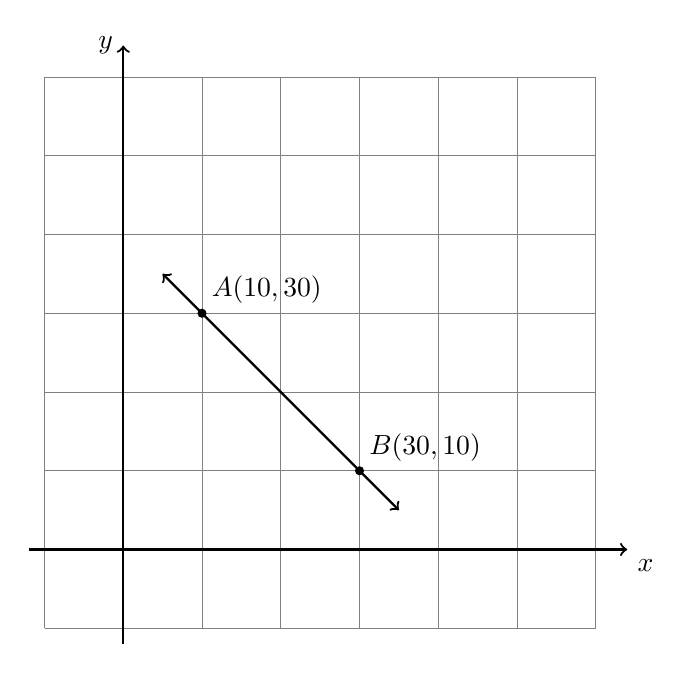
\begin{tikzpicture}[scale=1]
      \draw [help lines] (-1,-1) grid (6,6);
      \draw [thick, ->] (-1.2,0) -- (6.4,0) node [below right] {$x$};
      \draw [thick, ->] (0,-1.2)--(0,6.4) node [left] {$y$};
      \draw [fill] (1,3) circle [radius=0.05] node[above right] {$A(10,30)$};
      \draw [fill] (3,1) circle [radius=0.05] node[above right] {$B(30,10)$};
      \draw [<->, thick] (0.5,3.5)--(3.5,0.5);
    \end{tikzpicture}
    \end{flushright}
\end{multicols}

\newpage
\item Plot the points and find the slope of the line $\overleftrightarrow{RS}$, $R(20,10)$, $S(50,20)$. Use the formula and show the substitution step. As a check, draw the line and count the rise and run.
\begin{multicols}{2}
  $\displaystyle m = \frac{y_S - y_R}{x_S - x_R}$
    \vspace{2cm}
    \begin{flushright}
    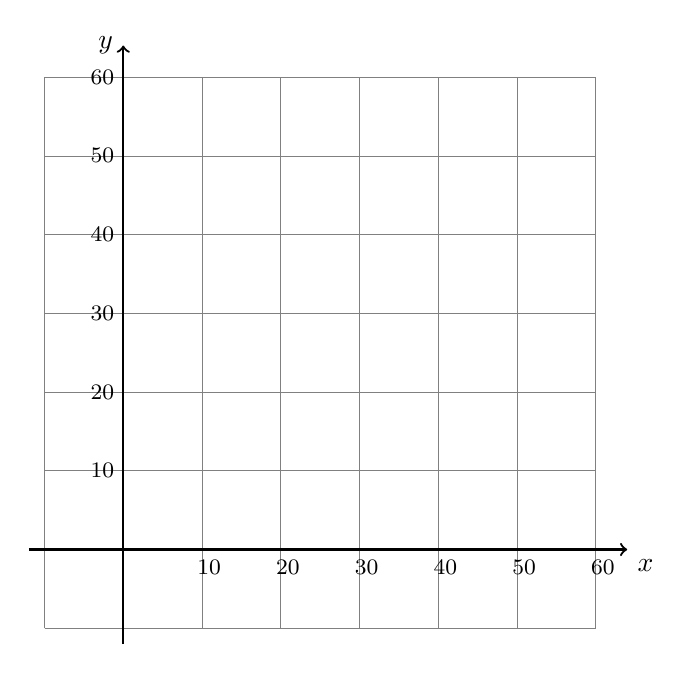
\begin{tikzpicture}[scale=0.1]
      \draw [help lines, xstep=10, ystep=10] (-10,-10) grid (60,60);
      \draw [thick, ->] (-12,0) -- (64,0) node [below right] {$x$};
      \foreach \x in {10,20,30,40,50,60}
        \draw[shift={(\x,0)},color=black] (0pt,2pt) -- (0pt,-2pt) node[below] {\footnotesize \; $\x$};
      \draw [thick, ->] (0,-12)--(0,64) node [left] {$y$};
      \foreach \y in {10,20,30,40,50,60}
        \draw[shift={(0,\y)},color=black] (-2pt,0pt) -- (2pt,0pt) node[left] {\footnotesize \; $\y$};
      %\draw [fill] (2,1) circle [radius=0.05] node[above left] {$A(2,1)$};
      %\draw [fill] (3,4) circle [radius=0.05] node[above right] {$B(3,4)$};
      %\draw [<->, thick] (1,-2)--(4,7);
    \end{tikzpicture}
    \end{flushright}
\end{multicols}

\newpage
\item Find the equation of the given line $\overleftrightarrow{AB}$, $A(0,40)$, $B(60,20)$.
\begin{multicols}{2}
    \begin{enumerate}[itemsep=1.2cm]
      \item Find the slope, $m$, showing the substitution step in the slope formula: \\[0.25cm]
      $\displaystyle m = (y_B - y_A)/(x_B - x_A)$
      \item Write down the $y$-intercept.
      \item Write the equation of the line.
      \end{enumerate}
      \begin{flushright}
        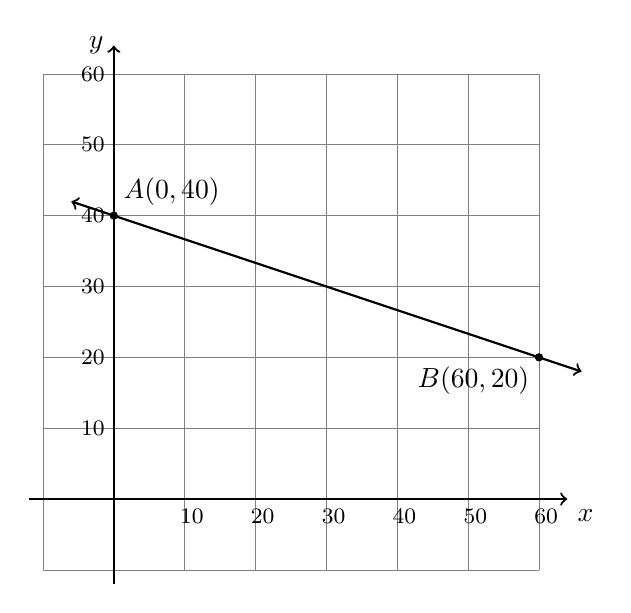
\begin{tikzpicture}[scale=0.09]
          \draw [help lines, xstep=10, ystep=10] (-10,-10) grid (60,60);
          \draw [thick, ->] (-12,0) -- (64,0) node [below right] {$x$};
          \foreach \x in {10,20,30,40,50,60}
            \draw[shift={(\x,0)},color=black] (0pt,2pt) -- (0pt,-2pt) node[below] {\footnotesize \; $\x$};
          \draw [thick, ->] (0,-12)--(0,64) node [left] {$y$};
          \foreach \y in {10,20,30,40,50,60}
            \draw[shift={(0,\y)},color=black] (-2pt,0pt) -- (2pt,0pt) node[left] {\footnotesize \; $\y$};
          \draw [fill] (0,40) circle [radius=0.5] node[above right] {$A(0,40)$};
          \draw [fill] (60,20) circle [radius=0.5] node[below left] {$B(60,20)$};
          \draw [<->, thick] (-6, 42)--(66,18);
        \end{tikzpicture}
        \end{flushright}
\end{multicols}

\newpage
\item Complete each statement about linear equations.
\begin{enumerate}[itemsep=0.5cm]
  \item What is the $y$-intercept of the line $y = 1.25x - 15.75$?
  \item What is the slope of the line $\displaystyle y = \frac{5}{2}x + 100$?
  \item Which has an zero slope, a vertical or horizontal line?
  \item What is the $y$-intercept of the line $\displaystyle y = \frac{3}{25}x + \frac{25}{3}$?

\end{enumerate}

\newpage
\item Is the point $C(60,30)$ on the line $l: y=\frac{1}{4}x+10$? \\[0.5cm]
Support your answer with \emph{both} algebra (substitute $C$'s coordinates into the equation) and geometry by graphing the line and point $C$.
\begin{flushright}
  \begin{tikzpicture}[scale=0.14]
    \draw [help lines, xstep=10, ystep=10] (-1,-1) grid (60,60);
    \draw [thick, ->] (-5,0) -- (64,0) node [below right] {$x$};
    \foreach \x in {10,20,30,40,50,60}
      \draw[shift={(\x,0)},color=black] (0pt,2pt) -- (0pt,-2pt) node[below] {\footnotesize \; $\x$};
    \draw [thick, ->] (0,-5)--(0,64) node [left] {$y$};
    \foreach \y in {10,20,30,40,50,60}
      \draw[shift={(0,\y)},color=black] (-2pt,0pt) -- (2pt,0pt) node[left] {\footnotesize \; $\y$};
    %\draw [fill] (2,1) circle [radius=0.05] node[above left] {$A(2,1)$};
    %\draw [fill] (3,4) circle [radius=0.05] node[above right] {$B(3,4)$};
    %\draw [<->, thick] (1,-2)--(4,7);
  \end{tikzpicture}
  \end{flushright}

\newpage
\item Write down the slope perpendicular to each slope (its negative reciprocal).
  \begin{enumerate}[itemsep=0.9cm]
    \item If $m = 3$ then $m_{\perp}=$
    \item If $\displaystyle m = -\frac{3}{2}$ then $m_{\perp}=$
    \item If $m = 4$ then $m_{\perp}=$
    \item If $\displaystyle m = -\frac{9}{4}$ then $m_{\perp}=$
  \end{enumerate}

\newpage
\item Quadrilateral $ABCD$ with vertices $A(2,5)$, $B(1,-1)$, $C(4,1)$, and $D(1,7)$ is shown. \\[0.5cm]
Find the slopes of each side. Is $ABCD$ a parallelogram? a rectangle? Justify your answer.
\begin{multicols}{2}
  Slope of $\overline{AB}=$\\[1.5cm]
  Slope of $\overline{BC}=$\\[1.5cm]
  Slope of $\overline{CD}=$\\[1.5cm]
  Slope of $\overline{AD}=$\\
  \begin{flushright}
    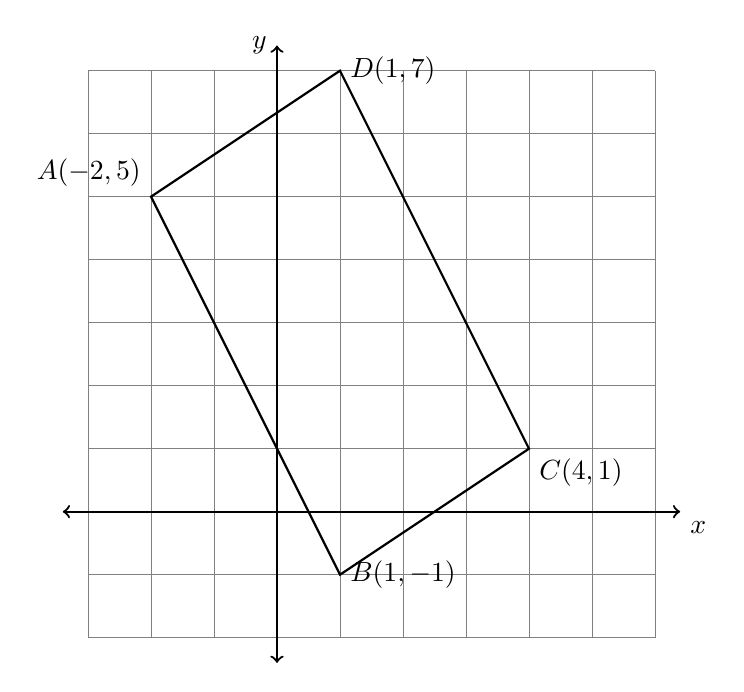
\begin{tikzpicture}[scale=0.8]
      \draw [help lines] (-3,-2) grid (6,7);
      \draw [thick, <->] (-3.4,0) -- (6.4,0) node [below right] {$x$};
      \draw [thick, <->] (0,-2.4)--(0,7.4) node [left] {$y$};
      \draw [thick] (-2,5) node[above left] {$A(-2,5)$}--
        (1,7) node[right] {$D(1,7)$}--
        (4,1) node[below right] {$C(4,1)$}--
        (1,-1) node[right] {$B(1,-1)$}--
        cycle;
    \end{tikzpicture}
    \end{flushright}
  \end{multicols}

\newpage
\item Plot a parallelogram (not a rectangle) using Geogebra (use the grid). The legs must not be horizontal or vertical. Paste an image of your work in this Classkick slide from the clipboard or by using the ``camera'' tool.\\[0.25cm]
Spicy: Show the measures the slopes of the quadrilateral sides.

  
\newpage
\item Complete the rectangle $ABCD$ on the graph, by adding the two missing sides.
\begin{multicols}{2}
    \begin{enumerate}[itemsep=2cm]
      \item Mark point $B$ on line $p$. Write the equation of line $\overleftrightarrow{AB}$.
      \item Mark point $D$ on line $q$. Write the equation of line $\overleftrightarrow{AD}$.
      \item Show that $\overleftrightarrow{AB} \perp \overleftrightarrow{AD}$ by showing that the product of their slopes is $-1$.
      \end{enumerate}
    \begin{flushright}
    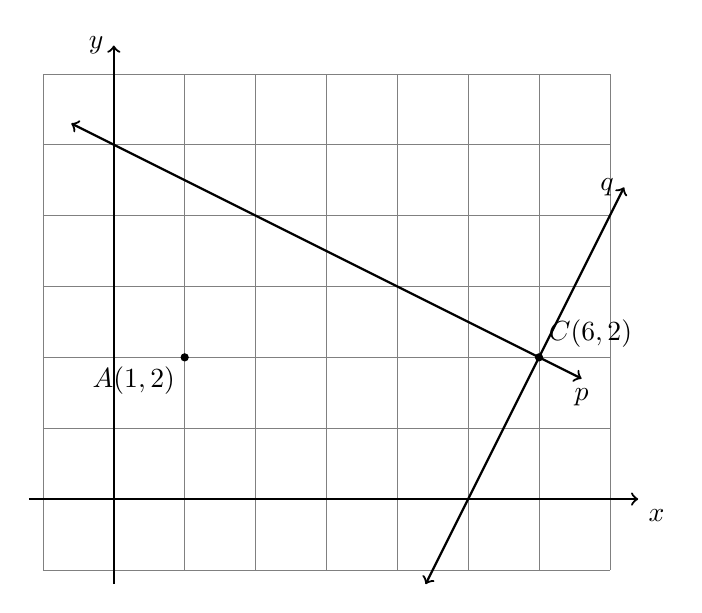
\begin{tikzpicture}[scale=0.9]
      \draw [help lines] (-1,-1) grid (7,6);
      \draw [thick, ->] (-1.2,0) -- (7.4,0) node [below right] {$x$};
      \draw [thick, ->] (0,-1.2)--(0,6.4) node [left] {$y$};
      \draw [fill] (1,2) circle [radius=0.05] node[below left] {$A(1,2)$};
      \draw [fill] (6,2) circle [radius=0.05] node[above right] {$C(6,2)$};
      \draw [<->, thick] (-0.6,5.3)--(6.6,1.7) node [below]{$p$};
      \draw [<->, thick] (4.4,-1.2)--(7.2,4.4) node [left]{$q$};
    \end{tikzpicture}
    \end{flushright}
\end{multicols}
    
\end{enumerate}
\end{document}

\newpage
\item A point labeled $C$ and vector $(1,3)$ are shown Geogebra/classic. Identify the following objects and tools.
  \begin{enumerate}
    \item Circle the vector
    \item Make an ``X'' where to click for the menu ``Name \& Value'' that will label point $C$ as an ordered pair.
    \item Mark with an arrow the menu where the ``Translate by vector'' tool is found.
  \end{enumerate}
  \begin{flushright}
    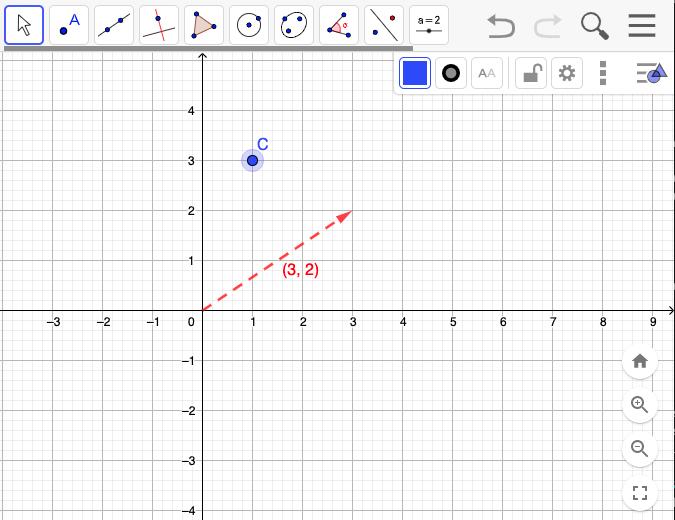
\includegraphics[width=6in]{5-11Geogebra_toolbar.png}
  \end{flushright}
